	\documentclass[a4paper,11pt, oneside]{book} \usepackage[czech]{babel}
	\usepackage[utf8]{inputenc}

	% Plugin na příkaz \say který udělá uvozovky
	\usepackage{dirtytalk}

	% Plugin na sloupce
	\usepackage{multicol}

	% Plugin na obrazky
	\usepackage{graphicx}
	\usepackage{wrapfig}

	% Toto je plugin diky kteremu pujde klikat do obsahu
	\usepackage{hyperref} \hypersetup{ colorlinks, citecolor=black,
	filecolor=black, linkcolor=black, urlcolor=black }

	% Plugin na hezci nadpis kapitoly
	% https://texblog.org/2012/07/03/fancy-latex-chapter-styles/
	\usepackage[T1]{fontenc} \usepackage{titlesec, blindtext, color}
	\definecolor{gray75}{gray}{0.75} \newcommand{\hsp}{\hspace{20pt}}
	\titleformat{\chapter}[hang]{\Huge\bfseries}{\thechapter\hsp\textcolor{gray75}{|}\hsp}{0pt}{\Huge\bfseries}


	% Zakladni info o dokumento
	\title{Ročníková práce} \author{Lukáš Dulík} \date{\today} % Tady sa pak moze nastavit jine datum, ted to da vzdycky aktualni


	% Plugin na zahlavi zapati
	\usepackage{fancyhdr}


	\fancyhf{} \lhead{Strojové učení} \lfoot{Ročníková práce KVARTA}
	\rfoot{\thepage}

	% Dulezite pro spravne zobrazovani zahlavi zapati
	\pagestyle{empty} \fancypagestyle{plain}{}

	\begin{document}

	% Zrusi cislovani na zacatecnich strankach
	\pagenumbering{gobble}

	\begin{titlepage} \begin{center} \vspace*{1cm}

			\Huge Gymnázium Jana Pivečky a Střední odborná škola Slavičín \\

			% Logo GJP
			
\includegraphics[width=0.4\textwidth]{img/gjp.png}

			\textbf{Ročníková práce}

			\vspace{0.5cm} \LARGE Téma: Strojové učení \end{center}

		\vspace{1.5cm}

		% Vyplni zbyvaji prostor
		\vfill

		\vspace{0.8cm}

		\vspace{5pt}
		% Cara nahore
		\hrule \vspace{6pt}

		\Large

		\makeatletter \begin{multicols}{2} \noindent Slavičín \\ Datum: \@date

		\columnbreak \noindent \null\hfill Třída: Kvarta \\ \null\hfill \@author
	\end{multicols}

		\makeatother

		\vspace{5pt}

		% Cara dole
		\hrule

	\end{titlepage}

	\newpage
		\mbox{}
	\newpage


	\noindent
	Prohlašuji, že jsem ročníkovou práci vypracoval samostatně
	a výhradně s použitím citovaných pramenů.


	\newpage
	\section*{Abstrakt}

	Strojové učení je mezi programátory známé ve své náročnosti, jelikož
	vyžaduje nejen dobré programovací schopnosti, ale také znalosti
	teoretické z oblastí lineární algebry, matematické analýzy a všeobecně tedy
	znalosti statistiky.
	Tato práce vás seznámí s metodami strojových učení a jejich využitím.
	Beru ji jako příležitost naučit se nějaké
	nové složitější způsoby řešení různých problémů, které bych pak mohl
	zakomponovat do mých programovacích a robotických projektů.

	\section*{Klíčová slova}

	programování, matematika, statistika, lineární algebra, matematická analýza, umělá inteligence, strojové učení



	\newpage
	\section*{Poděkování}
	Děkuji Ing. Tomáší Dulíkovi PhD za pomoc s prací a Jindřichu Maňasovi za pomoc s vykonáním praktické částí.

	% Udela obsah
	\tableofcontents

	\clearpage
	% Zacatek cislovani stranek
	\pagenumbering{arabic}
	\pagestyle{fancy}

	\chapter{Teoretická část}

	Od počátku výpočetních věků se programy rozhodovaly na základě jednoduchých,
	předdefinovaných logických podmínek. Postupem času ale začalo být potřeba
	vymýšlet dynamičtější způsoby rozhodování, umožňující práci s různorodými,
	dynamickými daty. Byli vymyšleny algoritmy a techniky umožňující programům učit
	se na základě dat, se kterými pracují. Většina dnes známých algoritmů byla
	vymyšlena někdy v druhé polovině 20. století, ale začla se
	používat ve velkém až na přelomu tisíciletí, kdy byl hardware
	dostatečně výkonný na tyto komplexní výpočetní modely.
	Tyto algoritmy využívají zejména statistické metody a lineární algebru.
	Obvykle se počítá s vektory, maticemi a obecně tedy s tenzory. Hardwarové
	implementace výpočtů, například jednotky GPU a TPU, mohou výpočty značně
	urychlit. Strojové učení se značně prolíná s oblastmi statistiky a datové
	analýzy. Má široké uplatnění ve všech oborech lidské činnosti díky tomu, že
	dokáže imitovat vždy nějakou malou část lidské inteligence. Nejenom, že může
	nahradit lidskou práci v činnostech, kde je potřeba mít něco konkrétního
	`naučené`, ale zároveň dosáhne rychlostí tisícinásobně větších než člověk.

	Nemůžeme ovšem strojové učení brát jako nějakou plnohodnotnou umělou superinteligenci.
	Zatím skládáme jenom kousky `inteligence` k sobě.
	Vždy jde jenom o kupu statistiky, která je vytvořena pro jednu určitou úlohu.
	Rozhodně nemůžeme tyto algoritmy srovnávat s lidským mozkem, který je mnohem,
	mnohem rozmanitější a schopnější. Sám se zvládá naučit,
	jak zvládnout jakékoli typy úloh a má dokonce
	nějaké interní podvědomí, o kterém ani pořádně nevíme, jak funguje. Lidský mozek je
	komplexní systém s dalekosáhlým záběrem. O umělém vybudování takové inteligence
	v počítači si zatím můžeme nechat jenom zdát.

	Strojové učení (Machine learning, ML) je důležitou součástí stále rostoucího oboru datových věd.
	ML algoritmy jsou stále více používány k odkrývání důležitých postřehů a informací uvnitř
	projektů dobývání znalostí. Postřehy ML systémů mají často důležitou váhu při klíčovém
	rozhodování ve větších korporacích. Poptávka o datových vědcích se stále zvyšuje.


	\section{Rozdělení algoritmů}

	Při \textbf{Učení pod dohledem}
	se programu dává učící datová sada, která obsahuje jak vstupy, tak požadované
	výstupy. Cíl programu je naučit se, jak obecně zmapovat vstupy na výstupy.
	Když program dojde k výsledným pravidlům, jde o něco, čemu říkáme model.
	Tento model by pak v ideálním případě měl jít aplikovat na jakékoli data stejného typu.


	Další typem algoritmů je \textbf{Učení bez učitele}. V tomto případě učící datová sada
	neobsahuje požadované výstupy. Vstupy tedy nejsou nijak označkované.
	Program musí sám najít nějaký způsob, jak strukturovat informace k sobě. Cíl
	je najít nějaké skryté obdobné vzory.

	Třetím typem je \textbf{Zpětnovazební učení}.
	Program pracuje v nějakém dynamickém prostředí, ve kterém musí splnit určitý
	cíl. Zpravidla jde o věci jako řízení auta na cestě nebo hraní hry proti
	protivníkovy.  Když ten úkol zkouší řešit, dostává zpětnou vazbu, která je
	úměrná tomu, jak dobře problémy zvládá. Cíl je tedy hodnotu této zpětné vazby
	maximalizovat.

	Byli vyvinuty i další metody strojového učení, které nespadají ani do jedné z
	těchto tří kategorií. V systémech je často kombinovánno víc způsobů dohromady.

	\subsection{Druhy úloh}

	V oblasti strojového učení můžeme úlohy a problémy rozdělit na tři základní typy.
	\textbf{Klasifikace} rozděluje vstupní data a zařazuje je do dvou a víc zadaných
		kategorií (tříd).  \textbf{Regrese} odhaduje číselnou hodnotu podle vstupu a známých výstupů. Dá se využít
	pro nejrůznější predikce. Patří k nejvýznamějším metodám matematické statistiky a
	používá se prakticky v každé oblasti aplikované vědy.
	\textbf{Shlukování} (clusterová analýza) hledá podobné vlastnosti objektů a následně je shlukuje do skupin.
	Narozdíl od klasifikace učící data nejsou označkované, a tak v nich musí program najít nějaký smysl
	sám.
	Cílem je, aby si jednotky náležící do skupin byli svými znaky podobnější než objekty z jiných
	skupin.
	Většinou se jedná o učení bez učitele.


	\section{Metody a algoritmy}

	V této sekci se pokusím vyzdvihnout nejpoužívanější metody a algoritmy.
	Oblast strojového učení a umělé inteligence se rozvíjí velmi rychle, stále
	jsou vymýšleny nové způsoby, a tak je těžké něco vypíchnout.


	\subsection{Regresní analýza}

	Jde o jednoduchou formu učení pod dohledem. Obecně jde o způsoby, jak dosadit
	nějakou přímku nebo křivku do grafu bodů. Snažíme se odhadnout hodnotu jisté
	náhodné veličiny (též cílová proměnná, regresand, či vysvětlovaná proměnná) se
	znalostí jiných veličin (nezávislých proměnných, vysvětlujích proměnných anebo
	kovariát).

	\begin{wrapfigure}{l}{0.5\textwidth} %this figure will be at the right
		\centering
		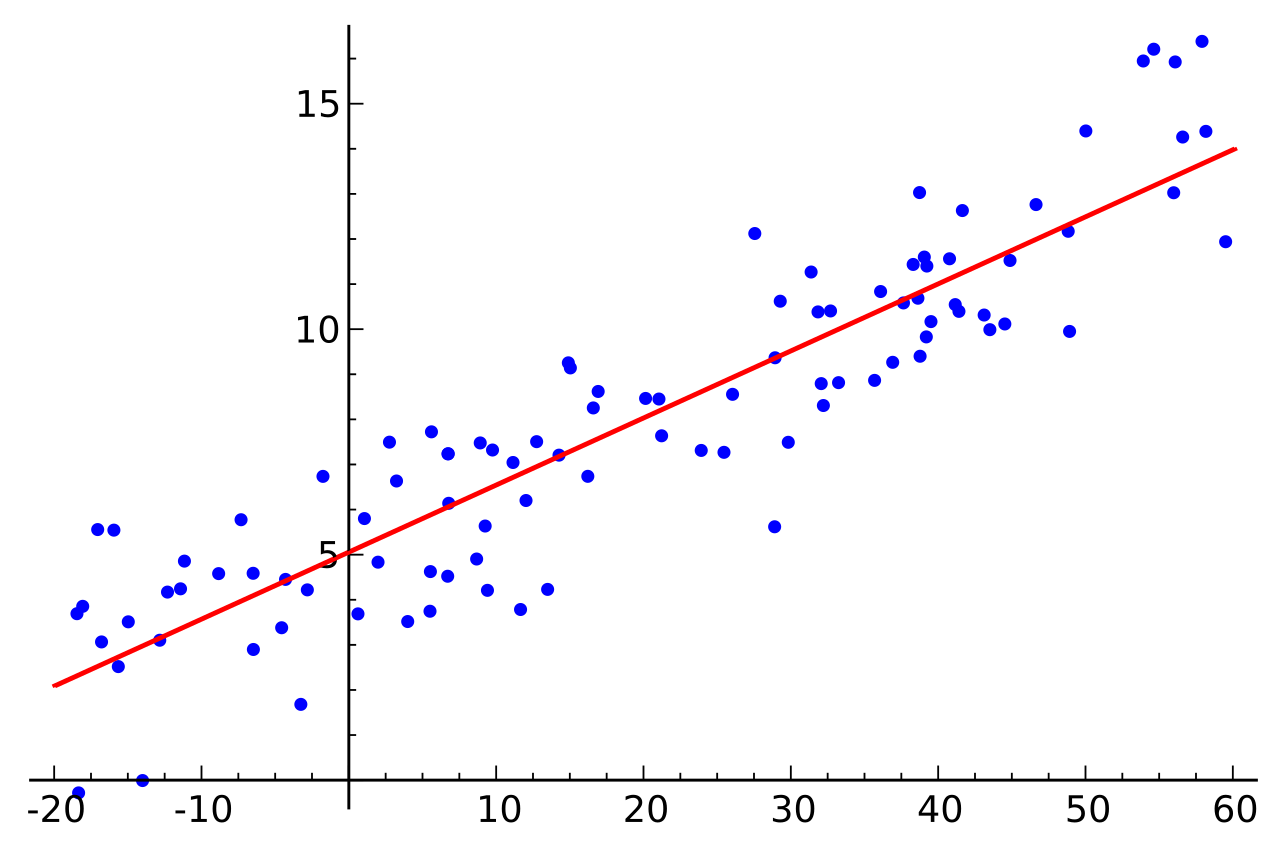
\includegraphics[width=0.5\textwidth]{img/linear-regression.png}
		\label{fig:linear-regression}
	\end{wrapfigure}

	Na základě podoby dat je nutno si zvolit, jaký typ regrese použít. Například,
	pokud víme, že mezi daty je lineární vztah, můžeme použít lineární regresi.
	Tato regrese představuje aproximaci daných hodnot přímkou.
	Pokud tuto přímku vyjádříme rovnicí \(y = mx + b\), jedná se o nalezení
	optimálních hodnot \(m\) a \(b\).

	Lineární regrese se nejčastěji počítá metodou nejmenších čtverců.
	Součet čtverců počítá sumu rozdílů bodů a hodnot dosazené přímky umocněných
	na druhou:

	\[ S(m,b) = \sum_{i=1}^n (mx_i + b - y_i )^2 \]

	Abychom minimalizovali tento součet čtverců, čili našli optimální koeficienty \(m\) a \(b\),
	použijeme následující vzorec. Na ten se dá přijít pomocí parciální derivace součtu čtverců a
	následnými úpravami soustavy rovnic.

	\[ m = \frac{n \sum x_i y_i - \sum x_i \sum y_i}{n \sum x_i^2 - (\sum x_i)^2 }\]

	\[ b = \frac{\sum x_i^2 \sum y_i - \sum x_i \sum x_i y_i }{n \sum x_i^2 - (\sum x_i)^2}\]

	Příklad použití lineární regrese může být třeba ve zmrzlinářství, které
	chce odhadnout počet prodaných zmrzlin podle dnešní venkovní teploty.
	Majitel si vede záznamy teplot a prodejů ,a tak může použít lineární regresi, aby
	přesně aproximoval dnešní počet prodejů.
	Data ale často nemají lineární podobu. Musíme pak použít nějakou složitější metodu regrese,
	která bude vhodná pro ten účel. Mezi další používané typy patří například mnohonásobná
	linární regrese, polynomiální regrese, logistická regrese, regrese s podpůrným vektorem
	a další.


	\subsection{Algoritmus k-nejbližších sousedů}

	Tato metoda byla poprvé vyvinuta v roce Evelynem Fixem and Josephem Hodgesem v roce 1951.
	Dá se použít pro regresi a klasifikaci.

	Pro hledání nejbližšího souseda v lze použít různé metriky.
	Nejobvyklejší je euklidovská metrika nebo Hammingova metrika.

	Příkladem použití tohoto algoritmu může být doporučovací systém, co na základě vašich
	hodnocení filmů najde \(k\) lidí (sousedů), kteří filmy zhodnotili co nejvíc podobně
	jak vy. Na základě toho vám doporučí filmy, co se jim líbily s předpokladem, že by se vám
	mohli líbit, protože máte s vašimi \say{sousedy} podobný vkus.


	\begin{wrapfigure}{r}{0.3\textwidth} %this figure will be at the right
		\centering
		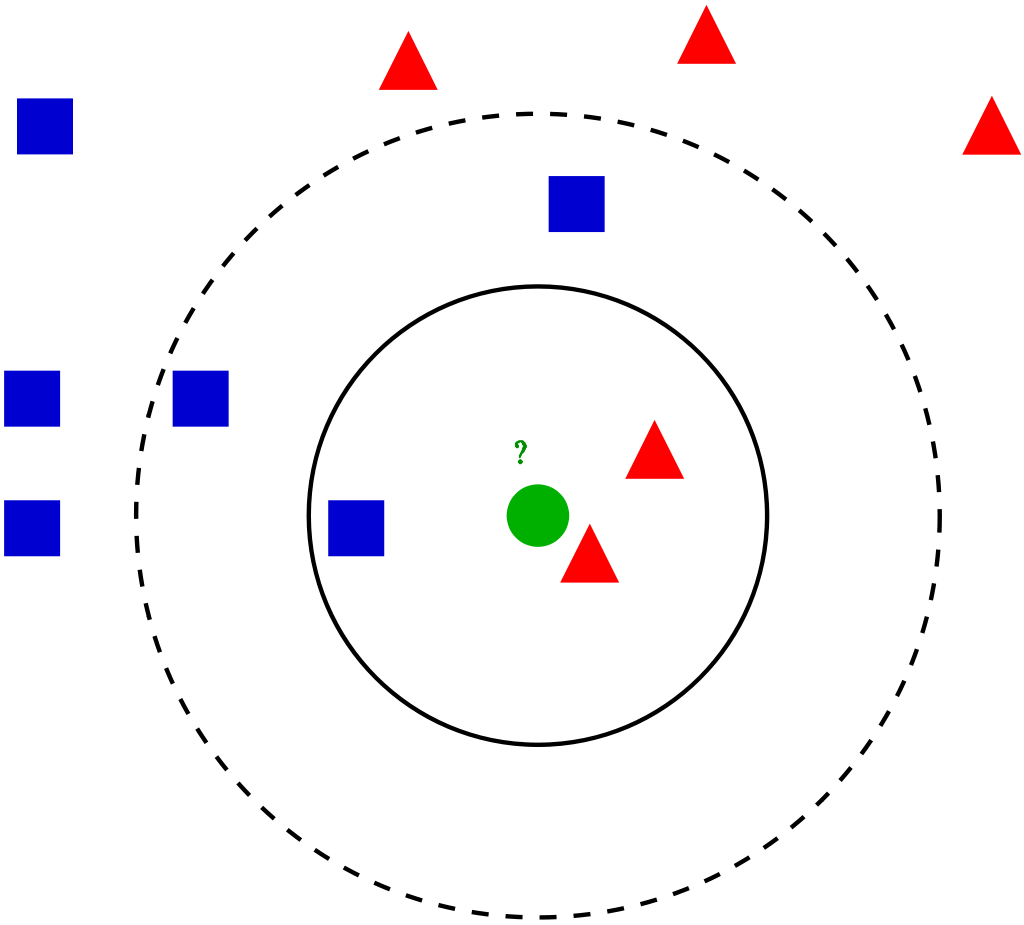
\includegraphics[width=0.2\textwidth]{img/knn-classification.png}
		\label{fig:knn-classification}
	\end{wrapfigure}

	Příklad použití za účelem klasifikace je k vidění na obrázku. Chceme klasifikovat
	zelený testovací vzorek buď k modrým čtvercům, nebo červeným trojúhelníkům na základě
	převažující skupiny k-nejbližších sousedů. Když by k bylo 3, byl by zařazen mezi
	červené trojúhelníky (kruh uvnitř). Když by k bylo 5, byl by zařazen mezi modré čtverce
	(čerchovaný kruh).

	Nevýhoda této metody je velká složitost, programy nejdou efektivně škálovat na vysoké množství dat.
	Taky nemá tolik různých využití, jako třeba neuronové sítě.

	\subsection{Neuronové sítě}

	Umělá neuronová síť je výpočetní model používaný v umělé inteligenci. Její způsob
	fungování je inspirován chováním odpovídajících biologických struktur. Skládá
	se z umělých neuronů, které jsou vzájemně propojeny. Navzájem si předávají signály a
	transformují je pomocí přenosových funkcí. Každý umělý neuron má určité množství vstupů
	a vychází z něho jeden výstup, který může být \say{poslán} do dalších neuronů.
	Vstupy neuronů mohou být nějaké charakteristiky nebo rysy externích dat, nebo
	vstupem může být výstup jiného neuronu. Výstupy konečných výstupních neuronů v sítí
	jsou výsledky řešení aktuálního zadání, jako třeba rozpoznání objektu v určitém obrázku.


	Existuje celá řáda modelů fungování umělých neuronů. Některé jsou jednoduché, některé
	se snaží co nejvíce napodobit fungování biologického organismu.
	Jedním z nejpoužívanějších je model popsaný v roce 1943 McCullochem a Pittsem.
	Pro zjištění výstupu neuronu nejpreve vezmeme sumu aktivací všech
	vstupních neuronů, váženou váhami spojnic ze vstupních neuronů do neuronu.
	K této sumě přádáme práh neuronu, který říká, jak moc musí být vážená suma
	velká aby se projevila na výstupu tohoto neuronu. Celá tato suma pak projde zvolenou
	přenosovou funkcí. Výsledný vzorec pak vypadá takto:

	\[Y = S(\sum_{i=1}^{N}(w_i x_i) + \Theta ) \]

	Kde \(x_i\) jsou vstupy neuronu, tedy aktivace čili výstupy neuronů napojených
	na tento neuron, \(w_i\) jsou váhy spojnic k tomuto neuronu, \(\Theta\) je práh tohoto neuronu,
	S(x) je přenosová funkce a \(Y\) je výstup neboli aktivace tohoto neuronu.

	Velikost vah \(w_i\) vyjadřuje uložení zkušeností do neuronů, které udává jak důležitý je daný vstup
	pro daný neuron. Práh \(\Theta\) označuje prahovou hodnotu aktivace neuronu


	Přenosová, též aktivační funkce, má za úkol hodnotu výstupu neuronu nějak zahladit, ořezat.
	Na obrázku můžete vidět grafy nejpoužívanějších aktivačních funkcí.

	\begin{figure}[h]
	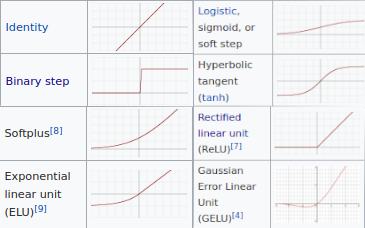
\includegraphics[width=0.6\textwidth]{img/activation-functions.png}
	\centering
	\end{figure}




	Neurony jsou organizovány různými způsoby. Typicky jsou rozděleny do vrstev, obvzlášť v oblasti
	hlubokého učení. Vrstvě, která příjmá externí data, říkáme vstupní vrstva. Vrstva, ze které vychází
	konečný výsledek sítě je výstupní vrstva.

	\begin{figure}[h]
	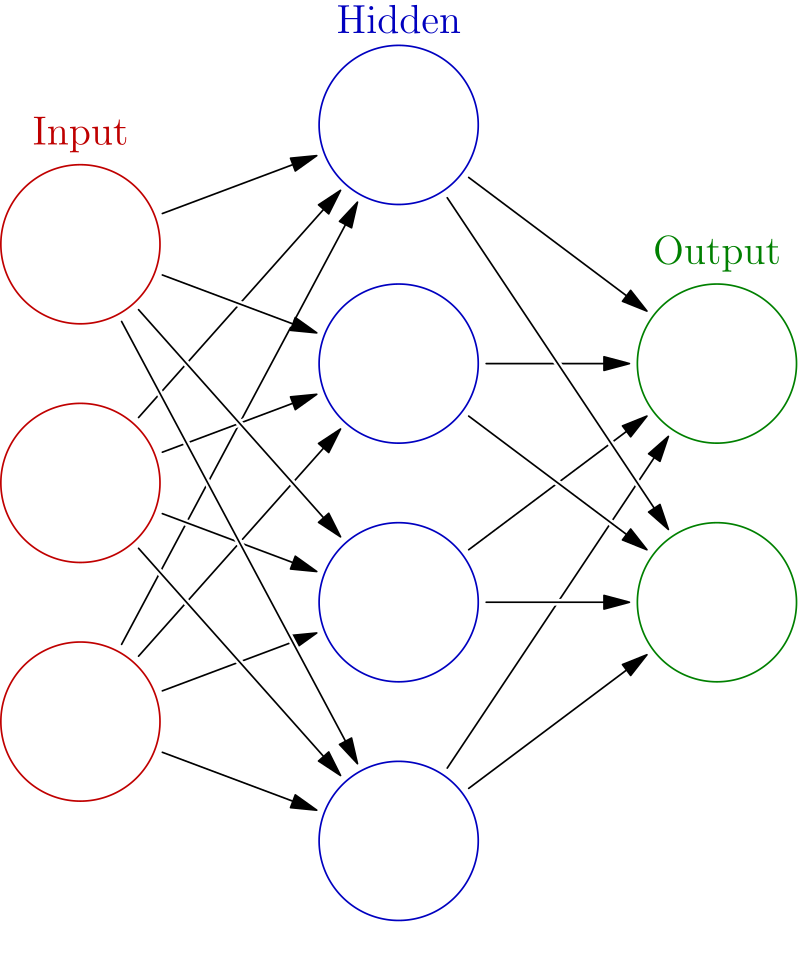
\includegraphics[width=0.5\textwidth]{img/Colored_neural_network.png}
	\centering
	\end{figure}


	Mezi nimi mohou být skryté vrstvy.
	Každý neuron ve vrstvě je spojen pouze s neurony v předchozí a následující vrstvě.
	Mohou být kompletně propojeny, což znamená, že neuron je propojen s každým neuronem v sousedních vrstvách.
	Takové síti říkáme vícevrstvý perceptron. Někdy se používají sítě, které určité spojení vynechávají, jako na obrázku.
	Sítě, které obsahují a povolují spojení mezi
	neurony ve stejných vrstvách a nesousedících vrstvách jsou známé, jako rekurentní neuronové
	sítě. V takové síti vznikají opakující se cykly.


	Kalkulace aktivací neuronů celé sítě může být vypočítána postupnou iterací, tedy
	tak, že postupně vypočítáme aktivaci každého neuronu v každé vrstvě. Tento postup se ale ve větších
	sítích ukáže jako časově velmi neefektivní, a je složité ho paralelizovat (rozdělit práci).
	Řešením je využít lineární algebru a počítat tak s více neurony naráz během jedné operace.
	Toto se nejlépe aplikuje na vícevrstvý perceptron (jednoduché vícevrstvé sítě).
	Neurony tak nereprezentujeme jednotlivě, ale ukládáme data o všech neuronech ve vrstvě.
	Pracujeme tak s vektorem aktivací \(x\) neuronů vrstvy \(i\), vektorem prahů \(\Theta\) vrstvy
	\(i\) a maticí spojnic \(w\) ke předchozí vrstvě \(i-1\). Na každý člen výsledného aktivačního
	vektoru aplikujeme přenosou funkci \(S(x)\).
	Aktivace všech neuronů ve vrstvě tak můžeme vypočítat v rámci jednoho jediného výrazu:

	\[Y_i = S(w_{i-1}  x_{i-1} + \Theta_i )\]

	Operace s maticemi a vektory se dobře paralelizují na vícero jader procesorů nebo GPU, které mají
	výpočetní jádra přímo pro tento účel. Knihovny často používají optimalizace, které je dělají ještě rychlejší.

	\subsubsection{Trénování}

	Nyní musíme zjistit optimální hodnoty všech vah a prahů, které dosáhnou požadované
	funkčnosti sítě. Jako první musíme použít nějaký způsob, jak zjistit celkovou
	kvalitativní funkčnost sítě. K tomu se používá nákladová funkce (cost function).
	Počítá se tak, že vždy vezmeme rozdíl aktivace a požadované aktivace výstupního neuronů,
	to celé umocníme na druhou. Suma všech těchto umocněných rozdílů je pak výstup cost funkce.
	Vektorový vzorec pak vypadá následovně. \(x_n\) je vektor aktivací výstupních neuronů,
	\(a\) je požadovaný vektor aktivací výstupních neuronů.
	\[ (x_n - a) ^ \top (x_n - a) \]

	O co vlastně v této funkci jde? Jde o mnohorozměrnou funkci, která má jako
	vstup nastavení naší sítě, tedy váhy a prahy, jako parametry může mít
	mnoho různých trénovacích příkladů dat a jako výstup jedno číslo (náklad).
	Naším cílem je toto číslo minimalizovat. Jak můžeme upravit nastavení vah a prahů tak,
	aby se náklad zmenšil, tím pádem, aby síť začala aspoň trochu fungovat?

	Musíme si představit nákladovou funkci jako nějaký prostor a zeptat se, jakým směrem se v tomto
	prostoru máme pohnout, abychom minimalizovali nákladovou funkci. Směr jsou
	změny vah a prahů.
	Který směr nejvíc zvýší náklad? Tomuto směru se říká gradient. Gradient určité funkci
	nám dává směr nejstrmějšího stoupání. Přirozeně, pohyb směrem záporného gradientu nám výstup nákladové
	funkce zmenší.

	A jak se takový gradient počítá? Pomocí matematické analýzy, konkrétně derivací, se dají
	z definice neuronu a nákladové funkce vyjádřit následující vzorce.

	V případě vícevrstvého perceptronu vyjádřeného pomocí lineární algebry se dají gradienty
	vypočítat takto. Výpočty jedou od poslední vrstvy dopředu vrstvu po vrstvě.
	Nejprve musíme v poslední vrstvě spočítat gradient vůči aktivacím.
	Jsou brány v potaz rozdíly skutečných a požadovaných aktivací.

	\[ \nabla_{a} C_L = 2 (x_L - y)\]

	Potom můžeme v každé vrstvě spočítat gradient prahů pomocí Hadamardova součinu.
	\(z_l\) jsou aktivace neuronů vrstvě předtím, než na ně byla aplikovaná přenosová funkce \(S\).
	\(S'\) znamená derivace funkce \(S\).

	\[ \nabla_\Theta C_l = \nabla_{a} C_l \odot S'(z_l) \]

	Poté gradient vah:

	\[ \nabla_w C_l = \nabla_\Theta C_l x_{l-1}^\top \]

	Před přechodem do další vrstvy musíme přepočítat gradient vůči aktivacím:

	\[ \nabla_{a} C_l = w_{l-1}^\top (S'(z_{l}) \odot \nabla_a C_{l+1})\]


	\begin{wrapfigure}{l}{0.5\textwidth} %this figure will be at the right
		\centering
		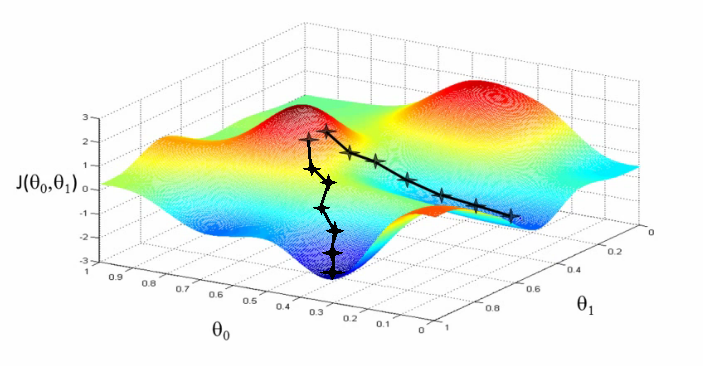
\includegraphics[width=0.5\textwidth]{img/gradient-descent.png}
		\label{fig:gradient-descent}
	\end{wrapfigure}

	Na obrázku vlevo můžete vidět vizualizaci klesání výstupu funkce pomocí výpočtu gradientu. V tomto případě
	má funkce jenom 2 vstupy a tak se dá výstup cost funkce vykreslit jako 3D plocha.
	Neuronové sítě mají vstupů mnohem víc, jedná se tak třeba o nějaký desetitisíc
	dimenzionální prostor, takže by cost funkce neuronové sítě vykreslit nešla.

	Když trénujeme síť pomocí aplikování gradientů, funkčnost sítě se zvyšuje a postupně se dostáváme
	k lokálnímu minimu výstupu nákladové funkce. Lokální minimum ale stále nemusí být ta nejefektivnější
	kombinace nastavení. Nejvíc kvalitní nastavení by udávalo globální minimum cost funkce.
	Bohužel ale neexistuje způsob, jak toto globální minimum najít.
	V trénovacích algoritmech se tak na konci trénování setkáváme s náhodným vyresetováním vah a
	prahů za účelem hledání nového lokálního minima z jiné pozice.

	Popsal jsem především fungování vícevrstvého perceptronu, ale je nutno podotknout,
	že existuje mnoho různých typů a podob neuronových sítí, které budou fungovat
	do určité míry jinak. Tento model je jeden z těch základních, ale zároveň už má
	sám o sobě mnoho různých využití.

	\subsubsection{Využití umělých neuronových sítí}

	Neuronové sítě mají mnoho aplikací. Používají se pro rozpoznávání a komprese obrazu a
	zvuku, rozpoznávání vzorů a sekvencí, strojový překlad, rozpoznávání spamů, virů a mnoho
	dalších věcí. V lékařství slouží k diagnostikám, byly použity k diagnóze
	několika druhů rakoviny a genetických vad. Ve finančnictví se používají pro
	automatické obchodování na burze. Taky byly široce zaměstnány v kybernetice,
	kde rozpoznávají škodlivé aktivity od těch legitimních.

	\subsection{Evoluční algoritmy}

	Genetický algoritmus je postup, který se snaží nalézt řešení složitých problémů,
	pro které neexistuje použitelný exaktní algoritmus, pomocí použití principů
	evoluční biologie. Pro `šlechtění` dané úlohy se používají techniky napodobující
	evoluční procesy. Jedná se o dědičnost, mutace, přirozený výběr a křížení.
	Princip spočívá v postupné tvorbě generací růzých řešení daného problému.
	Při řešení se uchovává populace, jejíž každý jedinec představuje jedno
	řešení problému. Při správné funkčnosti algoritmu se řešení zlepšují během
	průběhu evoluce. Typicky se první populace skládá z naprosto náhodných členů.
	Při přechodu do další generace je pro každého člena spočtena tzv. fitness funkce
	vyjadřující biologickou zdatnost, neboli cenu jedince z hlediska evoluce. Jedná se
	tedy o druh zpětnovazebního učení, kde zpětnou vazbu představuje tato fitness funkce.
	Pomocí tohoto hodnocení kvality jsou náhodně vybráni zdatnější jedinci,
	kteří jsou modifikování pomocí mutací a křížení. Vzniká tak nová populace.
	Tento postup se může opakovat na dobu neurčitou, čímž se kvalita řešení problému
	zvedá. Algoritmus se typicky zastaví, až když je kvalita populace dostačující,
	nebo po předem dáné době.

	Pro jedince se používá označení fenotyp a pro jeho reprezentaci se používá termín
	genotyp, genom nebo chromozom. Chromozom se skládá z jednotlivých genů,
	které jsou uspořádány v určitém pořadí. Nabývá různých hodnot, kterým se říká alely.
	Hodnoty mohou reprezentovat způsob, jakým jedinec řeší problém. Typicky jde
	o nějaké parametry řešení úlohy.

	Příkladovým použitím může být třeba program, co se sám snaží naučit hru Flappy bird.
	Ve hře se ovládá pták, který má za úkol proletět přes překážky. Kliknutím pták vyskočí.
	Pomocí evolučního algoritmu by se dal vytvořit program simulující evoluci ptáků s vlastní
	\say{inteligencí}. Chromozom každého jedince by mohl obsahovat informace o tom,
	v jakých vzdálenostech od překážek má skákat. První generace ptáků by měla
	tyto hodnoty nastaveny náhodně, a genetický algoritmus by hodnotil jejich schopnost podle
	toho, jak daleko se jim podařilo doletět. Potom by se vždy zdatnější ptáci vyfiltrovali
	a vykřížili a přešlo by se do další generace. Po pár generacích by byl umělý pták zdatnější,
	než normální hráč.



	\section{Využití}

	Strojové učení má mnoho různých využití. Pokusím se popsat, jaké jsou hlavní příklady použití
	v dnešním světě, ale taky, jaké použití se rozšíří v budoucnosti.

	Strojové učení je v největším rozsahu využíváno v systémech technologických gigantů.
	Pomocí vašeho dosavadního chování při konzumaci obsahu na internetových
	sítích dokážou \textbf{doporučovací algoritmy} odhadnout obsah, který by vás dokázal
	zaujmout na co nejdelší dobu. Toto je pro podnikání většiny gigantů více než
	relevantní, protože jejich zisk pohání především zobrazení cílených reklam
	přímo pro vás. Při používání sociálních sítí jejich systémy budují detailní profil
	vaší osoby, který pak dokáže odhadovat každý aspekt vašeho chovaní, za účelem
	zobrazení obsahu, který na síti udrží co nejdéle.
	Je znepokojivé, že osobní informace o vás, předně s detailní mapou vaší psychiky, je
	v rukou korporací. Jedná se tak o velmi kontroverzní použití této technologie.

	Akciový trh už dávno není o otevíracím zvonku a bílých američanech řvoucích po sobě
	v oblecích s kapsami plných peněz. Rychlost byla při obchodu vždy klíčová, a tak i
	ve finančnictví počítač docela rychle nahradil člověka. Ulice Wall Street dávno není
	plná lidí, co obchodují jménem firem. Nahradili je sytémy vysokofrekvenčního
	\textbf{algoritmického obchodování}. Je šílené pomyslet na to, že v podstatě celý západní burzovní
	trh stojí na sadě počítačů, které vykonávají tisíce obchodů
	za sekundu za účelem zvýšení svého vlastního portfolia.

	Strojové učení je zakomponováno do systémů \textbf{počítačového vidění}. Tyto technologie
	pak dokážou z obrázků nebo videí extrahovat smysluplné
	informace za pomocí konvolučních neuronových sítí. Počítačové vidění je
	aplikováno třeba v sociálních sítích, kde může automaticky označovat lidi na fotkách.
	Samoříditelné auta již nacházejí svou cestu na trh, a tak bude počítačové vidění
	stále více důležité i pro tyto účely. Své využití si našlo i ve zdravotnictví,
	kde může automaticky analyzovat výsledky rentgenů.
	K počítačovému vidění má blízko \textbf{rozpoznávání hlasu}. V mobilních zařízení bylo začleněno
	rozpoznávání hlasů do jejich systémů. Většinou se všechna zachycená
	slova rozpoznávají například na serverech Googlu, protože mobilní zařízení
	nemají požadovaný hardware na prácí s neuronovými sítěmi. Znepokojeně se tak opět
	dostáváme k otázce soukromí.

	Také můžeme kombinací mnoha algoritmů imitovat lidskou schopnost konverzovat.
	V zákaznických servisech se tak stále častěji můžeme setkat s robotem (chatbot) namísto
	člověka. Virtuální hlasoví asistenti, které si lidi pořizují domů, tohoto také využívají.

	Na \textbf{strojovém překladu} se dneska podílejí především komplexní algoritmy strojového učení.
	Programy se detailně učí jazyky a vznikají tak skoro perfektní překladatelé. Překladač Google
	nebo dokonce překladače vyvinuté na pražském Matfyzu dokáží pomocí složitých neuronových sítí
	perfektně přeložit většinu vět z angličtiny do češtiny a naopak.

	\section{Rizika a výzvy umělé inteligence}

	\textbf{Technologická singularita} je hypotetický zlomový bod technologického vývoje,
	v němž schopnosti umělé inteligence překonají schopnosti lidstva.
	Typickým scénářem technologické singularity je postavení počítače,
	který je schopen zkonstruovat dokonalejší počítač, aniž by si to lidstvo přálo.
	Výsledkem několika iterací tohoto procesu (rekurzivní sebevylepšení)
	by mohla být mocná umělá superinteligence,
	která by kvalitativně překonala veškerou lidskou inteligenci.
	Přestože toto téma přitahuje pozornost veřejnosti, většina výzkumníků tímto problému není
	znepokojena, protože se nezdá, že by takový typ inteligence měl být teď nebo v blízké době
	možný vyvinout.

	Další výzvou je \textbf{odpovědnost}.
	Když umělá mysl spáchá nějaký zločin, kdo za to ponese zodpovědnost? Samořízené auto
	může taky zavinit dopravní nehodu, i když je to mnohem méně pravděpodobné, než u lidského řidiče.
	Bude za nehodu zodpovědný řidič auta, to auto jako takové, nebo jeho výrobce?
	Probíhají diskuze, zda bychom měli
	prosazovat plně autonomní vozidla, nebo omezit výrobu pouze na semiautonomní vozidla.
	Semiautonomní vozidla zajišťují bezpečnost tvořenou řidičem, tím pádem přenáší odpovědnost na řidiče.
	Každá nová technologie vznese nějaké etické obavy. Toto jsou typy diskuzí, které probíhají
	a budou ještě častější při dalších průlomových objevech.

	Závažným problémem je také \textbf{soukromí}. Strojové učení potřebuje data, aby se mělo z čeho učit.
	Často jsou používány osobní data zákazníků, kteří k tomu vůbec nesvolili. Například v EU byla v roce
	2016 zavedena směrnice GDPR, která by takovému nesvolenému užití osobních údajů měla zabraňovat.




	\chapter{Praktická část}

	V rámci praktické části jsem se rozhodl naprogramovat dvě ukázky základních
	problémů strojového učení pod dohledem: regrese a klasifikace.

	\section{Demonstrace lineární regrese}

	\begin{wrapfigure}{r}{0.5\textwidth} %this figure will be at the right
		\centering
		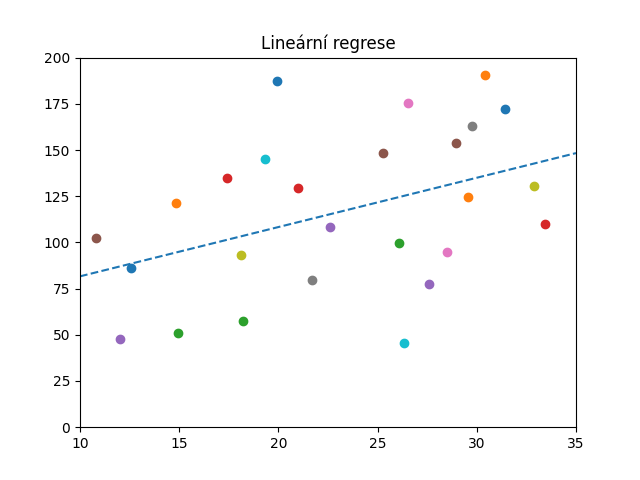
\includegraphics[width=0.5\textwidth]{img/linear-regression-demo.png}
	\end{wrapfigure}

	Pro ukázku regrese jsem vytvořil program vizualizující lineární regresi.  V
	tomto programu můžete klikáním přidávat datové body. Pomocí lineární regrese
	vždy vypočítá parametry přímky, která proloží všechny body z grafu. Tato přímka
	je pak vykreslena čárkovaně.  Pro implementaci jsem použil jazyk Python,
	protože je jednoduchý a má výbornou knihovnu matplotlib, která dělá
	vykreslování grafů záležitostí jednoho řádku.


	\section{Rozpoznávání číslic}

	Dále jsem naprogramoval klasifikační program číslic. Ve svém nitru používá
	záladní formu umělé neuronové sítě, vícevrstvý perceptron.  Chtěl jsem se naučit, jak fungují
	neuronové sítě, a tak jsem se rozhodl si ji naprogramovat sám. Rozpoznávání
	číslic jsem si zvolil, protože je to takový základní úkon v oblasti neuronových
	sítí. Díky tomu jsou na internetu volné datové sady označkovaných číslic. Já
	jsem si vybral volně dostupnou databázi MNIST od Národního institutu standardů
	a technologie USA, která obsahuje 60 000 trénovacích obrázků a 10 000
	testovacích obrázků v rozlišení 28 na 28 pixelů. Každý obrázek má k sobě
	informaci, o jakou číslici se doopravdy jedná.  Přemýšlel jsem, zda to udělat v
	Pythonu, nebo v C++ a nakonec jsem se rozhodl pro jazyk C++, a to kvůli
	rychlosti, přísnosti a uzpůsobilosti k objektově orientovanému programování.

	Myšlenka fungovaní neuronové sítě je celkem komplexní na pochopení. Pochopit to
	nebyla zrovna záležitost několika minut. Učil jsem se podle videí Granta
	Sandersona (3Blue1Brown) a každé video jsem si musel pustit několikrát znova,
	abych ten koncept nějak dostal do hlavy. Chtěl jsem, aby to fungovalo rychle,
	snažil jsem se každou část algoritmu zpracovávat pomocí lineární algebry.
	Například násobení matic a vektorů je mnohem rychlejší, než rekurzivní operace s
	každým neuronem, díky tomu, že jsou na to procesory i násobící algoritmy skvěle
	optimalizované. Na lineární algebru jsem si vybral knihovnu Eigen, která má
	typy pro vektory a matice a podporuje všechny operace. Přišla mi jako
	nejjednodušší knihovna na lineární algebru, její nevýhoda však je, že
	nepodporuje akceleraci výpočtů pomocí grafické karty. S matematickou
	interpretací trénovacího algoritmu za pomocí operací lineární algebry mi pomohl
	kamarád.

	\subsection{Implementace}
	Uspořádání programu jsem navrhl tak, že jsem vytvořil univerzální třídu neurové sítě,
	která obsahuje seznam vrstev neuronů. Každá vrstva je struktura obsahující
	vektor aktivací neuronů této vrstvy, vektor prahů neuronů této vrstvy a matici vah spojnic,
	kde n-tý řádek udává váhy spojnic k n-tému neuronu předchozí vrstvy. Dále pomocný obsahuje
	vektor a matici sloužící k ukládání sumy výsledků vah a prahů za každou trénovací dávku.

	Jako první jsem udělal funkci \textit{add\_layer(int size)}. Tato initializační funkce slouží k
	přidání vrstvy o \textit{size} neuronech. Díky tomu je moje třída neuronové sítě dynamická.
	Můžu si jednoduše změnit podobu celé neuronové sítě. V souboru main.cpp přidávám první
	vrstvu o 784 neuronech, protože mám data s tolika pixely. Skryté vrstvy používám dvě o velikostech
	16 a 16. Výstupní vrstva má 10 neuronů, protože rozpoznávám 10 různých číslic (0-9).
	Poté jsem vytvořil funkci \textit{calculate}, která vypočítá aktivace neuronů po celé síti. Pro
	každou vrstvu se vynásobí matice vah spojnic předchozí vrstvy s vektorem aktivací předchozí vrstvy
	a přičte se k tomu vektor prahů. Na to je aplikovaná lineární usměrňovací jednotka (ReLU).

	Nejsložitější bylo vymyslet funkci \textit{train\_on}. Tato funkce vezme parametr \textit{desired\_outcome},
	což je vektor žádoucích aktivací poslední vrstvy a na základě tohoto vektoru
	pomocí derivací a algoritmu zpětné propagace vypočítá gradient
	vah a gradient prahů. Gradienty jsou matice a vektor hodnot, které bychom na základě výsledků nynější
	trénovací iterace měli přičíst k matici vah a k vektoru prahů. Jsou vypočítány tak, aby
	minimalizovali hodnotu výstupu cost funkce, tím pádem zvýšili přesnost sítě.
	Tento gradient ale přímo ve funkci  nepřičítám, protože by to způsobovalo velké oscilace
	napříč trénovacími kousky, čímž by
	trénování fungovalo velmi nestabilně. Většinou se to řeší tak, že se aplikuje
	průměr těchto gradientů napříč x trénovacími kousky. Trénování tak funguje dávkově.
	V mojí funkci se gradienty přičítají k pomocnému dávkovému vektoru a matici.
	Funkci \textit{apply\_training\_batch} pak můžu zavolat, až v řídícím kódu
	natrénuji pár vzorků a ona pak vypočítá průměry gradientů a aplikuje jej na síť.

	Trénování ovládám tak, že vždy do aktivací vstupní vrstvy zapíšu hodnoty
	pixelů z obrázku z trénovacího datasetu, závolám funkci \textit{calculate}, následně
	\textit{train\_on} a po 20ti takovýchto obrázcích dám aplikovat dávku.
	Tímto způsobem projedu celý trénovací dataset a pak otestuji funkčnost sítě na
	testovacím datasetu. Pokud je rekordní, uložím si nynější hodnoty bokem. Poté vyresetuju
	váhy a prahy, náhodně je nastavím a celou trénovací operaci provádím znova.
	Program takto iteruje a zkouší to znova a znova na nových náhodných začátcích, dokud ho uživatel
	nezastaví. Toto náhodné resetování provádím, protože během té jedné trénovací iterace program najde
	nějaké lokální minimum cost funkce, ale toto lokální minimum většinou není globální, a tak je
	nutné začít znova na jiném místě a hledat nové lokální minimum s vírou v to, že bude menší, než
	ty předchozí. Až uživatel trénování zastaví, uloží nejlepší uložený model do souborů.

	\subsection{Výsledky}

	S touto neuronovou sítí se mi povedlo dosáhnout 95\% úspěšnosti. Tato úspěšnost by teoreticky
	šla ještě maximalizovat měněním podoby sítě, tedy změnou velikostí a počtu skrytých vrstev.
	Bohužel čím rozsáhlejší síť udělám, tím je trénování pomalejší. Nepodařilo se mi
	implementovat jednoduchý způsob, jak to počítat na GPU. To by trénování značně urychlilo.
	Kdybych tomu věnoval ještě nějaký čas, asi by se mi podařilo problémy s GPU vyřešit.
	Dále si jde hrát s parametrem míry učení a taky by šla změnit použitá přenosová funkce.


	\begin{wrapfigure}{l}{0.5\textwidth} %this figure will be at the right
		\centering
		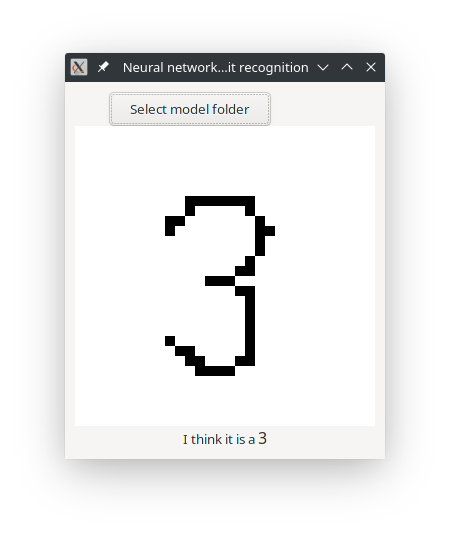
\includegraphics[width=0.4\textwidth]{img/neural-network-digit-gui.png}
	\end{wrapfigure}

	Na demonstraci funkčnosti jsem ještě zpětně doprogramoval GUI, kde můžete kreslit
	na plátno a neuronová síť odhaduje číslici, kterou kreslíte. Pro vytvoření
	grafického prostředí jsem použil knihovnu GTK. Při používání se někdy zdá, že neuronová
	síť nefunguje úplně dobře. To je hlavně tím, že byla natrénována na jinak vypadající
	obrázky s měkkými okraji pixelů. Síť pak může působit zmateně, když do ní dávám
	tyto tvrdě nakreslené obrazy.













	\chapter{Závěr}

	Strojové učení značně ovlivnilo náš svět. Díky němu se výrazně navýšilo množství úloh, které
	můžeme řešit pomocí počítačů. V některých oborech pomáhali systémy strojového učení
	tak efektivně a výhodně, že zcela nahradily práci lidí. Osobně si myslím, že strojové učení
	a obecně umělá inteligence jsou jedny z oborů budoucnosti. Bude potřeba víc a víc lidí vyvíjejících
	projekty s umělou inteligencí. Moje teorie je, že i většina programování co se vykonává dnes,
	typický databázový software pro firmy, kde je potřeba jenom zakomponovat nějakou jednoduchou
	byznys logiku, bude jednoho dne vykonávat umělá inteligence. Programátoři se tak přeorientují
	především na programování umělé inteligence. Otázka je, jestliže umělá inteligence
	a roboti nahradí práci tolika lidem, co budou pak ti lidé dělat? Někdo by namítl, že se jednoduše
	přeorientuje víc lidí na programování přímo té umělé inteligence. Já si právě myslím, že tak
	velká poptávka po lidech úplně nebude. Možná bude nutné
	trochu změnit způsob, jakým naše společnost a ekonomika funguje. To už je ale spíš otázka pro sociology.

	\chapter{Seznam použité literatury}

	\begin{enumerate}
	\item Bishop, C. M. (2006), Pattern Recognition
	and Machine Learning, Springer, ISBN 978-0-387-31073-2

		\item Mitchell, M.: An Introduction to Genetic Algorithms. Cambridge, MA: MIT Press 1996
	\end{enumerate}

	\chapter{Seznam odkazů}

	\begin{enumerate}
		\item Grant Sanderson - Neuronové sítě:
			\href{https://youtu.be/aircAruvnKk}{youtu.be/aircAruvnKk}
	% https://youtube.com/playlist?list=PLZHQObOWTQDNU6R1_67000Dx_ZCJB-3pi

		\item What is machine learning?
			\href{https://www.ibm.com/cloud/learn/machine-learning}{ibm.com/cloud/learn/machine-learning}

		\item What is Clustering?

			\href{https://developers.google.com/machine-learning/clustering/overview}{developers.google.com/machine-learning/clustering/overview}

		\item Regression analysis

			\href{https://en.wikipedia.org/wiki/Regression\_analysis}{https://en.wikipedia.org/wiki/Regression\_analysis}

		\item Linear regression

			\href{https://en.wikipedia.org/wiki/Linear\_regression}{https://en.wikipedia.org/wiki/Linear\_regression}

		\item K-nearest neighbors algorithm:

			\href{https://en.wikipedia.org/wiki/K-nearest\_neighbors\_algorithm}{en.wikipedia.org/wiki/K-nearest\_neighbors\_algorithm}

		\item Artifficial neural network
			\href{https://en.wikipedia.org/wiki/Artificial\_neural\_network}{en.wikipedia.org/wiki/Artificial\_neural\_network}

		\item Multilayer perceptron
			\href{https://en.wikipedia.org/wiki/Multilayer\_perceptron}{https://en.wikipedia.org/wiki/Multilayer\_perceptron}

		\item Activation function
			\href{https://en.wikipedia.org/wiki/Activation\_function}{en.wikipedia.org/wiki/Activation\_function}

		\item Gradient:
				\href{https://cs.wikipedia.org/wiki/Gradient\_(matematika)}{cs.wikipedia.org/wiki/Gradient\_(matematika)}

		\item Technologická singularita:

			\href{https://cs.wikipedia.org/wiki/Technologick\%C3\%A1\_singularita}{cs.wikipedia.org/wiki/Technologick\%C3\%A1\_singularita}

	\end{enumerate}

	\chapter{Seznam obrázků}

	\begin{enumerate}

		\item Example of simple linear regression, which has one independent variable
	https://commons.wikimedia.org/wiki/File:Linear\_regression.svg

		\item Example of k-NN classification
	By Antti Ajanki AnAj - Own work, CC BY-SA 3.0, https://commons.wikimedia.org/w/index.php?curid=2170282


		\item https://commons.wikimedia.org/wiki/File:Colored\_neural\_network.svg
	Glosser.ca, CC BY-SA 3.0 <https://creativecommons.org/licenses/by-sa/3.0>, via Wikimedia Commons

		\item Figure 3: Gradient Descent 3D diagram. Source: Coursera — Andrew Ng


	\end{enumerate}

	\chapter{Seznam příloh}

	\begin{enumerate}
		\item Klasifikační program číslic:
		\href{https://github.com/kukosek/neural-network-cpp}{github.com/kukosek/neural-network-cpp}

		\item Demo lineární regrese:
		\href{https://github.com/kukosek/rocnikovka}{github.com/kukosek/rocnikovka}
	\end{enumerate}
\end{document}

